\documentclass[runningheads]{llncs}
\usepackage{amsmath, amsfonts}
\usepackage{wrapfig}
\usepackage{tikz-qtree}
\usetikzlibrary{positioning}
\usetikzlibrary{arrows.meta}
\usetikzlibrary{arrows,shapes,quotes}
\usepackage[T1]{fontenc}
% T1 fonts will be used to generate the final print and online PDFs,
% so please use T1 fonts in your manuscript whenever possible.
% Other font encondings may result in incorrect characters.
%
\usepackage{graphicx}
% Used for displaying a sample figure. If possible, figure files should
% be included in EPS format.
%
% If you use the hyperref package, please uncomment the following two lines
% to display URLs in blue roman font according to Springer's eBook style:
%\usepackage{color}
%\renewcommand\UrlFont{\color{blue}\rmfamily}
%
\begin{document}
	%
	\title{Embedding Intuitionistic into Classical Logic}
	%
	%\titlerunning{Abbreviated paper title}
	% If the paper title is too long for the running head, you can set
	% an abbreviated paper title here
	%
	\author{Alexander Pluska \and Florian Zuleger}
	%
	\authorrunning{A. Pluska and F. Zuleger}
	% First names are abbreviated in the running head.
	% If there are more than two authors, 'et al.' is used.
	%
	\institute{TU Wien, Vienna, Austria}
	%
	\maketitle
\begin{abstract}
The famous double negation translation~\cite{glivenko1929quelques,godel1933intuitionistischen} establishes an embedding from classical into intuitionistic logic. Curiously the reverse direction has not been covered in literature. Based on the work in~\cite{claessen2015sat} we establish a small model property for intuitionistic propositional logic which allows us to utilize its Kripke semantics to give a simple embedding into classical propositional logic and quantified boolean formulas. We then transfer this procedure to first-order logic which allows us to give a embedding of intuitionistic first-order logic into classical first-order-logic.

%The key notion used in the proofs is the existence of counter-models - an analogon to the satisfiability of the negation in classical logic, which is not equivalent to invalidity in the intuitionistic case.  We hope that this will allow leveraging the tremendous recent progress in automated reasoning in classical logic for checking intuitionistic validity, for which there has not been much progress in recent decades.

This allows a direct application of state-of-the-art classical first-order provers to the problem of determining intuitionistic validity. A first benchmark shows that our approach is competitive. Crucially, our constructions support the transfer of counter-models to validity, which is important to model checking applications, where the output of counter-examples is an appreciated feature.
\end{abstract}

\section{Introduction}


Constructive mathematics refers to a flavour of mathematics in which the existence of an object can only be established by explicit construction, as opposed to classical mathematics where existence can be shown implicitly, e.g. by assuming non-existence and deriving a contradiction.
The formalism usually associated with constructive mathematics is intuitionistic logic, which essentially differentiates itself from classical logic by the fact that the law of excluded middle $A\vee\neg A$ and the double negation shift $\forall x\neg\neg P(x)\to\neg\neg\forall xP(x)$ are not valid.
Besides philosophical considerations, most prominently advocated by Brouwer~\cite{brouwer1907over} and Bishop~\cite{bishop1967foundations}, there is a particular motivation for studying constructive mathematics from the perspective of computer science in that proofs in  intuitionistic logic directly correspond to computer programs --- as expressed in the Curry--Howard correspondence~\cite{howard1980formulae}.

The interest in intuitionistic logic has lead to the development of a number of automated theorem proving systems for propositional as well as for predicate logic and a collection of benchmark problems (see e.g. the ILTP library website~\cite{iltp}).
However, intuitionistic provers perform poorly compared to their classical counterparts, see e.g. the TPTP~\cite{casc} and SAT~\cite{satc} competitions.
%, e.g., the first-order provers~\cite{kovacs2013first, schulz2002brainiac, korovin2008iprover}
%Comparing benchmarks for classical and intuitionistic automated theorem proving, e.g. TPTP~\cite{casc} and , we see that classical provers currently have a far better success rate. Furthermore all the most popular first-order utilize classical logic.
This difference can be partially explained by fundamental differences between the logics.
First of all, determining intuitionistic validity is computationally harder, i.e. in the propositional case intuitionistic validity is \verb+PSPACE+-complete~\cite{statman1979intuitionistic} whereas classical validity is \verb+coNP+-complete~\cite{cook1971complexity}.
A further advantage of classical logic is the existence of calculi that are particularly suitable for automation such as superposition~\cite{bachmair2001resolution}, which rely on the existence of convenient normal forms such as CNF, and the duality between validity and satisfiability, i.e. to show the validity of a formula it suffices to show the unsatisfiability of the negated formula, which is insufficient in intuitionistic logic.
The first dedicated intuitionistic theorem provers~\cite{mclaughlin2009efficient,tammet1996resolution} used the naive inverse method, i.e. direct search for a cut-free proof by applying the rules from some proof calculus inversely, which generally leads to a very complex search. More recently connection-based methods have been applied to various non-classical logics~\cite{otten2005clausal,otten2021nanocop}, including intuitionistic logic, and show promise.
There have also been some successful attempts to study intuitionistic validity via embedding into higher-order classical logic~\cite{LEO}.
Finally, we add that in contrast to intuitionistic provers a tremendous amount of work has been put into optimizing provers for classical logic.

With this work we want to examine a new but evident approach for directly leveraging the progress in classical reasoning for intuitionistic logic.
To this end, we give an embedding from intuitionistic logic into classical logic. That is, we give an effective procedure that returns for each formula $\varphi$ a modified formula $\varphi^\#$, such that $\varphi$ is intuitionistically valid if and only if $\varphi^\#$ is classically valid.
Interestingly, the reverse direction, the famous double-negation translation, has long been established and goes back to Glivenko~\cite{glivenko1929quelques} in the propositional case, and to G\"odel~\cite{godel1933intuitionistischen} and Gentzen~\cite{gentzen1936widerspruchsfreiheit} in the first-order case. In the propositional case it is particularly simple: $\varphi$ is classically valid if and only if $\neg\neg\varphi$ is intuitionistically valid. Intuitively the translation collapses for each subformula $\psi$ of $\varphi$ the truth values of $\psi$ and $\neg\neg\psi$, which are classically but not intuitionistically equivalent. This gives us a first idea why the reverse direction is perhaps more difficult: We need to expand the truth values of $\psi$ and $\neg\neg\psi$, i.e. if they both occur in $\varphi$, we must have a way to (classically) assign different truth values to their respective counterparts in $\varphi^\#$. In particular, this necessitates the introduction of new propositional variables in our procedure, which already marks a big difference to the double negation translation.
%
In addition to the translation of formulas we give an effective translation of counter-models, i.e. for each intuitionistic counter-model of $\varphi$ we can effectively construct a classical counter-model of $\varphi^\#$ and vice versa.
We note that the existence of counter-models is a key notion that forms a proper dual to validity --- whereas the satisfiability of the negation is not necessary for invalidity (in contrast to classical logic, where it is a proper dual to validity).
Transforming and reducing counter-models to a normal form is also what ultimately enables our translation.

In summary, our work suggests the following approach:
\begin{itemize}
	\item performing our translation on the input formula $\varphi$ to obtain $\varphi^\#$,
	\item checking the classical validity of $\varphi^\#$ with the prover resulting in a proof or counter-model,
	\item translating the proof/counter-model of $\varphi^\#$ to a (intuitionistic) proof/counter-model of $\varphi$.
\end{itemize}


\section{Preliminaries}

In this section we fix notation and recall the semantics for classical and intuitionistic logic. Futhermore we recapitulate some results from~\cite{otten2005clausal}.

\subsection{Propositional Semantics}

\begin{definition}
	A \emph{valuation} $v$ maps each propositional variable $A$ to a \emph{truth value} $v(A)\in\{0, 1\}$. We inductively define the model relation $\models$ between $v$ and formulas:
	\begin{itemize}
		\item $v\not\models \bot$, $v\models A$ iff $v(A) = 1$ for each propositional variable $A$.
		\item $v\models \varphi\wedge\psi$ iff $v\models\varphi$ and $v\models\psi$.
		\item $v\models\varphi\vee\psi$ iff $v\models\varphi$ or $v\models\psi$.
		\item $v\models\varphi\to \psi$ iff $v\not\models\varphi$ or $v\models\psi$.
	\end{itemize}
	A valuation $v$ is a \emph{model} for $\varphi$ if $v\models\varphi$. If every valuation is a model for $\varphi$ then we say $\varphi$ is \emph{valid}. We denote the set of valid formulas with \emph{CPC} (Classical Propositional Calculus).
\end{definition}

One notable property of classical logic is that a formula $\varphi$ is valid if and only if its negation $\neg\varphi := \varphi\to\bot$ is not satisfiable, i.e. there does not exist a model for it. The same does not hold true for intuitionistic logic as we shall see.

\begin{definition}
	A \emph{Kripke structure} $\mathcal K = (W, (v_w)_{w\in W})$ consists of a partially ordered set $W$ of \emph{worlds}, called the Kripke \emph{frame}, and a family of valuations $(v_w)_{w\in W}$ such that $v_u(A)\leq v_u(A)$ for all $u\leq w$ and propositional variables $A$ (this is called the \emph{persistency condition}).
	The model relation between the $v_u$ and formulas $\varphi$ is defined as before, except in the case of implications, where we set
	\begin{itemize}
		\item $v_u\models\varphi\to \psi$ iff for all $w\geq u$ we have $w\not\models\varphi$ or $u\models\psi$.
	\end{itemize}
	We say that $\varphi$ is satisfied at a world $u$ if $v_u\models\varphi$ and write $u\models\varphi$. If a formula is satisfied at every world then $\mathcal K$ is a \emph{model} for $\varphi$. A formula is valid if every Kripke structure is a model of it. We denote the set of valid formulas with \emph{IPC} (Intuitionistic Propositional Calculus).
\end{definition}
There are many classical tautologies which are not intuitionistically valid, e.g. the law of excluded middle $A\vee\neg A$. On the other hand any intuitionistic theorem is a classical one.

\subsection{Predicate Semantics}

We now recall the semantics of first-order logic:

\begin{definition}
	Let $\Sigma$ be a signature. A $\Sigma$-structure $\mathcal{M}$ consists of a non-empty set $M$, the \emph{domain} of $\mathcal{M}$, and an \emph{interpretation} $I$ that assigns
	\begin{itemize}
		\item to each $n$-ary function symbol $f$ a $n$-ary function $f^I: M^n\to M$.
		\item to each $n$-ary relation symbol $R$ a $n$-ary relation $R^I\subseteq M^n$.
	\end{itemize}
	A variable assignment $v$ is a function that assigns to each free variable an element $m\in M$. For each free variable $a$ and $m\in M$ we define $$v[m/a](b) = \begin{cases}
	m, &\text{if $b=a$,}\\
	v(b), &\text{otherwise.}
	\end{cases}$$
	Then terms are interpreted as follows:
	\begin{itemize}
		\item $a^{I, v} = v(a)$ for each free variable $a$.
		\item $f(t_1,\dots,t_n)^{I, v} = f^I(t_1^{I, v},\dots, t_n^{I, v})$.
	\end{itemize}
	We define a model relation between pairs $\mathcal M, v$ and formulas $\varphi$ as follows
	\begin{itemize}
		\item $\mathcal M, v\not\models\bot$
		\item $\mathcal M, v\models R(t_1,\dots,t_n)$ iff $(t_1^{I, v},\dots,t_n^{I, v})\in R^I$, $\mathcal M, v\models s = t$ iff $s^{I, v} = t^{I, v}$.
		\item $\mathcal M, v\models \varphi\wedge \psi$ iff $\mathcal M, v\models\varphi$ and $\mathcal M, v\models\psi$
		\item $\mathcal M, v\models \varphi\vee\psi$ iff $\mathcal M, v\models\varphi$ or $\mathcal M, v\models\psi$.
		\item $\mathcal M, v\models \varphi\to\psi$ iff $\mathcal M, v\not\models\varphi$ or $\mathcal M, v\models\psi$.
		\item $\mathcal M, v\models\exists x\varphi$ iff there exists $m\in M$ such that $\mathcal M, v[m/a]\models\varphi[a/x]$ where a is a free variable that does not occur in $\varphi$.
		\item $\mathcal M, v\models\forall x\varphi$ iff for all $m\in M$ we have $\mathcal M, v[m/a]\models\varphi[a/x]$ where a is a free variable that does not occur in $\varphi$.
	\end{itemize}
	$\varphi$ is satisfiable if there exist $\mathcal M, v$  with $\mathcal M, v\models\varphi$. A $\Sigma$-structure $\mathcal M$ satisfies $\varphi$ if $\mathcal M, v\models\varphi$ for every $v$, we write $\mathcal M\models\varphi$. A formula is valid if every $\Sigma$-structure $\mathcal M$ satisfies it. We denote the set of valid formulas with \emph{CQC} (Classical Quantified Calculus).
\end{definition}

\begin{definition}
	A $\Sigma$-\emph{Kripke structure} $\mathcal{K}$ is a partially ordered set $W$, called the Kripke \emph{frame}, and a family of $\Sigma$-structures $(\mathcal{M}_w)_{w\in W}$ such that for $u\leq w$ we have $M_u\subseteq M_w$, $f^{I_w}|_{M_u} = f^{I_u}$ and $R^{I_w}|_{M_u} = R^{I_u}$.\footnote{Here $f|_M$ denotes the restriction of $f$ to $M$}
	The model relation between $\mathcal M_u$, $v$ (targeting $\mathcal M_u$) and formulas $\varphi$ is defined as before, except in the cases of implication and $\forall$-quantification, where we set
	\begin{itemize}
		\item $\mathcal M_u, v\models \varphi\to\psi$ iff for every $w\geq u$ we have $w, v\not\models\varphi$ or $w, v\models\psi$.
		\item $\mathcal M_u, v\models\forall x\varphi$ iff for every $w\geq u$ and $m\in M_w$ we have $w, v[m/a]\models\varphi[a/x]$ where a is a free variable that does not occur in $\varphi$.
	\end{itemize}
	We write $u, v\models\varphi$ if $\mathcal M_u, v\models \varphi$. $\mathcal{K}$ satisfies $\varphi$ if $u, v\models\varphi$ holds for every world $u$ and variable assignment $v$. If such $\mathcal K$ exists then $\varphi$ is satisfiable. $\varphi$ is valid if it is satisfied by every Kripke structure.
	$\varphi$ is valid for some frame (write $W\models\varphi$) if it is satisfied in every Krike structure with that frame. We denote the set of valid formulas with \emph{IQC} (Intuitionistic Quantified Calculus).
\end{definition}
In addition to the propositional tautologies there are now sentences involving quantifiers which are classically valid but not intuitionistically, e.g., $\neg\forall x A(x)\to \exists x \neg A(x)$.

\subsection{Skolemization and Herbrandization}\label{section:herbrandiaztion}

An important step in the embedding will be the elimination of quantifiers via Herbrandization.
In this process we introduce fresh variables and add additional function symbols to the signature.
A fresh variable is any variable that does not occur in any of the considered formulas.
Whenever we add a function symbol we implicitly extend the signature by some not previously contained symbol.

\begin{definition}
	For formulas $\varphi$ we define the Skolemization $\varphi^S_Z$ and Herbrandization $\varphi^H_Z$ with respect to $Z$ by simultaneous induction as follows:
	\begin{itemize}
		\item $A^S_Z = A^H_Z = A$ for each atomic $A$.
		\item $(\varphi\circ\psi)^X_Z = \varphi^X_Z\circ\psi^X_Z$ for $\circ\in\{\wedge, \vee\}$, $X\in\{S, H\}$.
		\item $(\varphi\to\psi)^S_Z = \varphi^H_Z\to \psi^S_Z$\\$(\varphi\to\psi)^H_Z = \varphi^S_Z\to\psi^H_Z$.
		\item $(\forall x\varphi)^S_Z = \forall x(\varphi[a/x]^S_{Z\cup\{a\}}[x/a])$ where $a$ is a new free variable\\$(\forall x\varphi)^H_Z = \varphi[s(z_1,\dots,z_n)/x]^H_Z$ where $s$ is a new function, $\{z_1\dots z_n\} = Z$.
		\item $(\exists x\varphi)^S_Z = \varphi[s(z_1,\dots,z_n)/x]^S_Z$ where $s$ is a new function, $\{z_1\dots z_n\} = Z$\\$(\exists x\varphi)^H_Z = \exists x(\varphi[a/x]^H_{Z\cup\{a\}}[x/a])$ where $a$ is a new free variable.
	\end{itemize}
	Let $\varphi^S = (\exists x_1\dots\exists x_n \varphi[x_1/a_1\dots x_n/a_n])^S_\emptyset$ and $\varphi^H = (\forall x_1\dots\forall x_n \varphi[x_1/a_1\dots x_n/a_n])^H_\emptyset$ where $a_1,\dots,a_n$ are the free variables occurring in $\varphi$.
\end{definition}

\begin{theorem}
	\label{thm:herbrand-skolem}
	For every formula $\varphi$
	\begin{itemize}
		\item $\varphi$ and $\varphi^S$ are classically equisatisfiable.
		\item $\varphi$ and $\varphi^H$ are classically equivalid.
	\end{itemize}
\end{theorem}

Theorem~\ref{thm:herbrand-skolem} follows from Lemmata~\ref{ap1} and~\ref{ap2} stated in the appendix.

\subsection{Intuitionistic normal forms}

Finally we note the results from~\cite{otten2005clausal} which are of importance to us.

\begin{lemma}\label{lemma:propositional-normal-form}
	For every propositional formula $\varphi$ there exists an atom $P$ as well as sets of clauses $\mathcal R, \mathcal X$, with $\mathcal R$ containing  \emph{flat clauses} of the form
	$$\bigwedge_iA_i\to\bigvee_jB_j$$
	and $\mathcal X$ containing \emph{implication clauses} of the form
	$$(A\to B)\to C,$$
	such that $\varphi$ is intuitionistically equivalid to
	$$\left(\bigwedge\mathcal R\wedge\bigwedge\mathcal X\right)\to P$$where $A_i, B_i, A, B, C$ are atomic. The size of $\mathcal R$ and $\mathcal X$ is linear in the size of $\varphi$. In general they will contain additional propositional variables.
\end{lemma}

A similar result holds in the first order case.

\begin{lemma}\label{lemma:first-order-normal-form}
	For every predicate formula $\varphi$ there exists a nullary relation symol $P$ as well as sets of clauses $\mathcal R,\mathcal X, \mathcal Q$, with $\mathcal R$ containing \emph{flat clauses} of the form
	$$\forall \vec x\left(\bigwedge_i A_i\to \bigvee_jB_j\right),$$
	$\mathcal X$ containing \emph{implication clauses} of the form
	$$\forall \vec x\left((A\to B)\to C\right)$$
	and $\mathcal Q$ containing \emph{quantification clauses} of the form
	$$\forall\vec x\left((\forall y A)\to B\right),$$
	such that $\varphi$ is intuitionistically equivalid to
	$$\left(\bigwedge\mathcal R\wedge\bigwedge \mathcal X\wedge\bigwedge\mathcal Q\right)\to P$$where $A_i, B_i, A, B, C$ are atomic. This size of $\mathcal R, \mathcal X, \mathcal Q$ is linear in the size of $\varphi$. In general this formula will contain new function and relation symbols.
\end{lemma}

Since we could not find a proof of this result one is given in the appendix as Lemma~\ref{proof:first-order-normal-form}.

\section{Overview}

We shall now give an overview of our main results and highlight the key arguments. Recall that our goal is to give an effective translation procedure that, for a given formula $\varphi$, yields a formula $\varphi^\#$, such that $\varphi$ is intuitionistically valid if and only if $\varphi^\#$ is classically valid. We start with the propositional case. The key arguments are the same as in the first-order case, while it is technically simpler and less cluttered.

Before our main transformation we employ a preprocessing step akin to the Tseytin transformation~\cite{tseitin1983complexity}, which is a popular pre-processing step in classical automated reasoning:
It gives an equisatisfiable sentence (over an extended set of propositions) in conjunctive normal form.
Eliminating all implications, however, is not possible in intuitionistic logic since $A\to B$ is not equivalent to $\neg A\vee B$.
Still we propose a similar transformation.
A notable feature of our transformation is that all non-classical content is encapsulated in formulas of type $(A\to B)\to C$, i.e. if there are no such formulas in the transformed formula then the classical validity of the transformed formula immediately implies intuitionistic validity.

\begin{theorem}\label{thm:Tseytin}
For every propositional formula $\varphi$ there effectively are an atom $P$ and a set of $\mathcal S$ of formulas (over an extended set of propositions) of one of the forms\\
$\hspace{1cm} A\to (B\wedge C), (A\wedge B)\to C, A\to (B\vee C), (A\vee B)\to C, (A\to B)\to C,$\\
for atomic $A, B, C$, such that $\varphi$ is intuitionistically valid if and only if $\bigwedge\mathcal S\to P$ is intuitionistically valid. The time complexity of the transformation is linear in the input size.
\end{theorem}

The main transformation then proceeds in three steps:
%
1) We encode as a first-order sentence that the considered formula holds for every Kripke frame.
Since Kripke frames for propositional logic over a fixed alphabet of propositional variables form a first-order theory this step is rather straightforward.
%
2) Next we eliminate some quantifiers via Herbrandization. The only quantifiers eliminated occur in formulas derived from formulas of type $(A\to B)\to C$.
%
3) We can then argue that if there is a counter-model for the resulting formula then there is a counter-model with a certain Kripke frame of bounded size completely determined by the number of formulas of type $(A\to B)\to C$.
This allows us to eliminate the remaining quantifiers by simply enumerating the worlds in that Kripke frame.

Summarizing, we obtain the following result:

\begin{theorem}
\label{thm:reduction-propositional}
	Let $\mathcal S$ be as in Theorem~\ref{thm:Tseytin} and $\mathcal F_\to\subseteq\mathcal S$ denote the subset of formulas of the form $(A\to B)\to C$ and $\Lambda$ denote the set of sequences without repetition over $\mathcal F_\to$. For each atom $A$ and $k\in\Lambda$ consider a new atom $A^k$. Obtain $\mathcal S^\#$ by including the following formulas:
	\begin{itemize}
		\item $A^k\to A^{k\psi}$ for each atom $A$ occurring in $\mathcal S$, $k\in\Lambda$ and $\psi\in\mathcal F_\to$ not occurring in $k$.
		\item $A^k\to (B^k\circ C^k)$ for each $\circ\in\{\wedge,\vee\}$, $A\to (B\circ C)\in\mathcal S$, $k\in\Lambda$.
		\item $(A^k\circ B^k)\to C^k$ for each $\circ\in\{\wedge,\vee\}$, $A\to (B\circ C)\in\mathcal S$, $k\in\Lambda$.
		\item $(A^{k\psi}\to B^{k\psi})\to C^k$ for $\psi = (A\to B)\to C\in\mathcal S$, $k\in\Lambda$ if $\psi$ does not occur in $k$.
	\end{itemize}
Then, $\bigwedge S\to P$ is intuitionistically valid iff $\bigwedge S^\#\to P^\epsilon$ is classically valid, where $\epsilon$ denotes the empty sequence. The size of $\mathcal S^\#$ is in $\mathcal O(|\mathcal S|\cdot2^{|\mathcal F_\to|\cdot\log(|\mathcal F_\to|)})$. Futhermore, there is an effective procedure for translating counter-models between the sentences.
\end{theorem}

Instead of explicitly enumerating the worlds of a counter-example of bounded size (as in the reduction stated in the above theorem), we can also do this enumeration implicitly with a quantified boolean formula (QBF).
We can show that this QBF is satisfiable if and only if there exists a counter-model for our original formula:

\begin{theorem}
	Let $\mathcal S$ be as in Theorem~\ref{thm:Tseytin} and $\mathcal F_\to\subseteq\mathcal S$ denote the subset of formulas of the form $(A\to B)\to C$. There is an effective procedure that produces a QBF $\varphi^Q$ of size $\mathcal O(|\mathcal S|\cdot|\mathcal F_\to| + |\mathcal F_\to|^3)$ with $2\cdot |\mathcal F_\to|-1$ quantifier alternations such that $\varphi$ is intuitionistically valid if and only if $\varphi^Q$ is not satisfiable. For fixed $N\in\mathbb N$, deciding intuitionistic validity for formulas $\bigwedge \mathcal S\to P$ where $\mathcal S$ is as above and $|\mathcal F_\to| = N$ is therefore in $\Sigma_{2N-1}$.
\end{theorem}

%\begin{theorem}
%	For every predicate formula $\varphi$ there exists an effective procedure that yields an atom $P$ and a set $\mathcal S$ of formulas of the forms
%	$$\forall \vec z(A(\vec a)\to (B(\vec b)\wedge C(\vec c))), \forall \vec z((A(\vec a)\wedge B(\vec b))\to C(\vec c)),$$$$\forall \vec z(A(\vec a)\to (B(\vec b)\vee C(\vec c))),
%	\forall \vec z((A(\vec a)\vee B(\vec b))\to C(\vec c)),$$$$ \forall \vec z((A(\vec a)\to B(\vec b))\to C(\vec c)),\forall \vec z(\forall xA(\vec a)\to B(\vec b)),$$$$ \forall \vec z(A(\vec a)\to\forall xB(b)), \forall \vec z(\exists xA(\vec a)\to B(\vec b)), \forall \vec z(A(\vec a)\to\exists xB(b))$$for atomic $A, B, C$ and vectors of variables $\vec z, \vec a, \vec b, \vec c$ such that $\varphi$ is intuitionistically valid if and only if $\bigwedge\mathcal S\to P$ is intuitionistically valid. The size of $\mathcal S$ and time complexity of the transformation are linear in the input size.
%\end{theorem}

We then move to the first-order case. Here the construction is a bit more involved but the underlying approach is the same.
Again we first perform a Tseytin-like transformation.
Here the non-classical content is encapsulated by formulas of type $(A\to B)\to C$ and $\forall xA\to B$.
The details of this translation are given in Section~\ref{section:tseytin}.
We then proceed similarly to the propositional case.
Note however that one difficulty arises from the fact that our (classical) domain will now contain on the one hand worlds in the Kripke frame but on the other hand also proper domain elements.
We resolve this apparent conflict by introducing a special binary predicate $E$, inspired by~\cite{iemhoff2010eskolemization}, encoding which domain elements exists at which world.
The main transformation then again proceeds in three steps:
Step 1) and 2) are analogous to the propositional case.
The real difference arises in step 3):
While we can also establish the existence of a canonic counter-model whose frame only depends on formulas of type $(A\to B)\to C$ and $\forall xA\to B$, the size of this counter-model is countably infinite in general.
This is not surprising since certain intuitionistically invalid formulas like the double negation shift $\forall x\neg\neg A(x)\to \neg\neg\forall x A(x)$ don't have finite counter-models.
Therefore we are not able to eliminate the $\forall$-quantifiers associated with the Kripke semantics.
However since our translation targets first-order logic, we believe that the introduction of these quantifiers is acceptable.
%
Summarizing, we obtain the following result:

\begin{theorem}
\label{thm:reduction-first-order-short}
There exists a linear-time procedure that gives for every first-order formula $\varphi$ a formula $\varphi^\#$ such that $\varphi$ is intuitionistically valid if and only if $\varphi^\#$ is classically valid. The size of $\varphi^\#$ is in linear in the size of $\varphi$, however, for each $n$-ary relation symbol in $\varphi$ there is a corresponding $n+1$-ary relation symbol in $\varphi^\#$, and $\varphi$ contains a new binary predicate $E$ as well as a number of new function symbols. Furthermore, there is an effective translation between intuitionistic counter-models of $\varphi$ and classical counter-models of $\varphi^\#$.
\end{theorem}
A more detailed account of Theorem~\ref{thm:reduction-first-order-short} is given in Theorem~\ref{thm:fo-translation}.

These results provide an effective framework for using classical provers to check intuitionistic validity. First experiments with the Vampire theorem prover~\cite{kovacs2013first} show promise.




\section{Bounded Intuitionistic Counter-models}

The most obvious approach to embedding intuitionistic into classical logic is to examine intuitionistic semantics, e.g. Kripke frames, as a classical first order theory. For every propositional variable $A$ consider a unary predicate $A$ of the same name where $A(u)$ expresses that $A$ is true at some world $u$. We can then consider the following naive encoding:

\begin{definition}
	Let $\varphi$ be a propositional formula. Define $\varphi^{u}$ inductively:
	\begin{itemize}
		\item $\bot^u = \bot$.
		\item $A^{u} = A(u)$ for every propositional variable $A$.
		\item $(\varphi\circ\psi)^u = \varphi^u\circ\psi^u$ for $\circ\in\{\wedge, \vee\}$.
		\item $(\varphi\to \psi)^u = \forall w(u\preceq w\to\varphi^{w}\to\psi^{w})$ where $w$ is some new variable.
	\end{itemize}
	Let $K(\varphi)$ encode the theory of Kripke structures, i.e.
	$$K(\varphi) = \text{\normalfont PartialOrder}(\preceq)\wedge\forall u\forall w(u\preceq w\to \text{\normalfont Persistent}(u, w))$$
	with e.g.
	\begin{align*}
		\text{\normalfont PartialOrder}(\preceq) =&\:\forall u(u\preceq u)\wedge\forall u\forall w(u\preceq w\to w\preceq u\to u = w)\wedge\\&\:\forall u\forall v\forall w(u\preceq v\to v\preceq w\to u\preceq w)\\
		\text{\normalfont Persistent}(u, w)=&\:\bigwedge \{A(u)\to A(w)\:|\: \text{ $A$ occurs in $\varphi$}\}
	\end{align*}
	Then define
	$$\varphi^{C} = K(\varphi)\to \forall u\varphi^{u}.$$
\end{definition}

\noindent As all we have done is modeling Kripke frames as a first-order theory so we directly obtain:

\begin{lemma}
	$\varphi$ is intuitionistically valid if and only if $\varphi^C$ is classically valid.
\end{lemma}

This is somewhat unsatisfying as we end up in a much more complex logic. However using the normal form from Lemma~\ref{lemma:propositional-normal-form}, i.e. assuming that $\varphi$ is of the form $$\left(\bigwedge\mathcal R\wedge\bigwedge\mathcal X\right)\to P$$ for some flat clauses $\mathcal R$ and implicational clauses $\mathcal X$, further simplification is possible:
\begin{itemize}
	\item For flat clauses $(\bigwedge A_i\to\bigvee B_j)^u$ is
	$$\forall w\left(u\preceq w\to\bigwedge_i A_i(w)\to\bigvee_jB_j(w)\right).$$
	\item For implication clauses $((A\to B)\to C)^u$ is
	$$\forall w(u\preceq w\to(\forall k(w\preceq k\to A(k)\to B(k)))\to C(w))$$
\end{itemize}

and after applying Herbrandization we end up with a formula $$\varphi^{CH} = K(\varphi)\to\left(\bigwedge\mathcal R^{uS}\wedge \bigwedge\mathcal X^{uS}\right)\to P(s)$$ where $s$ is a new constant symbol, each formula in $\mathcal R^{uS}$ is of the form
$$\forall w\left(s\preceq w\to\bigwedge_iA_i(w)\to\bigvee_jB_j(w)\right)$$
and each formula $\psi\in\mathcal X^{uS}$ is of the form
$$\forall w(s\preceq w\to(w\preceq f_\psi(w)\to A(f_\psi(w))\to B(f_\psi(w)))\to C(w))$$
with $f_\psi$ being a new function symbol.

We now argue that if a counter-model for $\varphi^{CH}$ exists then a small counter-model exists. This is ultimately what enables our translations.

\begin{definition}
For $\psi\in\mathcal X$ let $[\psi]$ denote the corresponding clause in $\mathcal X^{uS}$. Suppose we are given a counter-model $\mathcal M = (M, I)$ for $\varphi^{CH}$.
We say $(A\to B)\to C\in\mathcal X$ is \emph{fulfilled} at $m\in M$ iff $A^I(m)\to B^I(m)$ is false or $C^I(m)$ is true. For $\psi\in\mathcal X$ define $$g_\psi : M\to M, m\mapsto\begin{cases}
		m,&\text{ if $\psi$ is fulfilled at $u$,}\\
		f^I_{\lbrack\psi\rbrack}(m),&\text{ else.}		
	\end{cases}$$Define a model $\mathcal M_T = (M_T, I_T)$ as follows:
	\begin{itemize}
		\item $M_T$ is the set of sequences without repetition on $\mathcal X$.
		\item $s^{I_T} = \epsilon$.
		\item Interpret $\preceq$ as the prefix-order.
		\item We set $$f_\psi^{I_T}(\psi_1\dots\psi_n) = \begin{cases}
			\psi_1\dots\psi_n, &\text{if $\psi$ occurs in $[\psi_1]\dots[\psi_n]$,}\\
			\psi_1\dots\psi_n\psi, &\text{else.}			
		\end{cases}$$
		\item For propositional variables $P$, we set $$P^{I_T}\left(\psi_1\dots \psi_n\right) = P^I\left(g_{\psi_n}\left(\dots\left(g_{\psi_1}\left(s^I\right)\right)\dots\right)\right).$$
	\end{itemize}
\end{definition}
\begin{lemma}~\label{thm:prop-countermodel-reduction}
	Let $\mathcal M = (M, I)$ be a counter-model to $\mathcal \varphi^{CH}$.
	\begin{enumerate}
		\item $\psi$ is fulfilled at $f_{[\psi]}^I(u)$ for all $u\in M, \psi\in\mathcal X$.
		\item If $\psi$ is fulfilled at some $m\in M$ then $\psi$ is fulfilled at all $n\succeq m$.
	\end{enumerate}
\end{lemma}

A proof can be found in the appendix as Lemma~\ref{proof:prop-countermodel-reduction}. Essentially what this tells us is that for every $m$ at which $\psi$ is fulfilled, in particular for each $m$ in the image of $f_{[\psi]}$, we may add the assumption that $f_{[\psi]}(n) = n$ for all $n\geq m$ without changing the validity of $\psi$.
With this lemma in hand showing that $(M_T, I_T)$ is a counter-model to $\varphi^{CH}$ is a straightforward check of definitions.

\begin{corollary}\label{cor:prop-tree-model}
	If $\mathcal M$ is a counter-model to $\varphi^{CH}$ then so is $\mathcal M_T$.
\end{corollary}

An example of this translation can be found in the appendix as Example~\ref{ex:prop-tree-model}.

\begin{remark}
	It is well known that Kripke frames which are trees are complete with regard to intuitionistic logic. Our contribution is giving an easy to compute explicit size and geometry that depends only on the structure of the considered formula.
\end{remark}

\begin{corollary}
	If a formula in normal form as in Lemma~\ref{lemma:propositional-normal-form} in intuitionistically invalid then there exists a Kripke counter-model which is a rooted tree with height and degree bounded by $|\mathcal X|$.
\end{corollary}

\section{IPC to CPC}

We can apply the previous results to give a direct embedding from intuitionistic into classical propositional logic. We know that $\varphi^{CH}$ is valid iff it is valid for structures that have as a domain the sequences without repetition over $\mathcal F_\to$, ordered by the prefix-relation and $$s^I = \epsilon, f_\psi^I(x) = \begin{cases}
	x, &\text{ if $\psi$ occurs in $x$,}\\
	x\psi, &\text{ otherwise.}
\end{cases}$$
Now we can replace every $\forall$-quantifier in $\varphi^{CH}$ by enumerating all the ground terms, and then replace all distinct ground instances of relations by new propositional variables yielding a propositional formula. Note that the encoding of partial order becomes redundant with this so we drop it, but we need to keep the persistency constraints. This gives us the following theorem:

\begin{theorem}
	Suppose we are given a formula as in Lemma~\ref{lemma:propositional-normal-form}, i.e. of the form
	$$\left(\bigwedge\mathcal R\wedge\bigwedge\mathcal S\right)\to P$$
	with flat $\mathcal R$ and implication $\mathcal S$. Let $\Lambda$ denote the set of sequences without repetition over $\mathcal X$. For every propositional variable $A$ and $\lambda\in\Lambda$ consider a new propositional Variable $A^\lambda$. Define $R^\#$ as the union over all sets
	$$
		\left\{\bigwedge_iA_i^\lambda\to\bigvee_jB_j^\lambda\:|\:\lambda\in\Lambda\right\}
	$$
	for $\bigwedge_iA_i\to\bigvee_jB_j\in\mathcal R$ and $\mathcal X^\#$ as the union over all sets
	$$
		\left\{\left(A^{\lambda\psi} \to A^{\lambda\psi}\right)\to(C^\lambda)\:|\:\lambda\in\Lambda, \psi\text{ does not occur in }\lambda\right\}
	$$
	for $\psi = (A\to B)\to C\in\mathcal X$ as well as $P^\#$ as the union over all sets
	$$
		\left\{A^\lambda\to A^{\lambda\psi}\:|\:\lambda\in\Lambda, \psi\psi\text{ does not occur in }\lambda\right\}
	$$
	 for each propositional variable $A$ occurring in $\varphi$ encoding persistency. Then
	$$
		\varphi^\# := \left(\bigwedge P^\#\wedge\bigwedge \mathcal R^\#\wedge\bigwedge\mathcal X^\#\right)\to P^\epsilon
	$$
	is classically valid if and only if $\varphi$ is intuitionistically valid.
\end{theorem}
%\begin{theorem}
%	$\bigwedge\mathcal S\to P$ is intuitionistically valid iff $\bigwedge\mathcal S^\#\to P^\emptyset$ is classically valid.
%\end{theorem}

\begin{example}
	Let us consider the law of excluded middle $\varphi = A\vee\neg A$ for which there is the equivalid normal form
	$$((A\to P)\wedge ((A\to \bot)\to P))\to P.$$
	Applying the above lemma this is intuitionistically valid if and only if $$((A^\epsilon\to A^\psi)\wedge(P^\epsilon\to P^\psi)\wedge(A^\epsilon\to P^\epsilon)\wedge(A^\psi\to P^\psi)\wedge ((A^\psi\to \bot)\to P^\epsilon))\to P^\epsilon$$ is classically valid where $\psi := (A\to \bot)\to P$.
	We note that $A^\epsilon  = P^\epsilon = 0$, $A^\psi = P^{\psi}  = 1$ indeed defines a counter-model.
\end{example}	

\section{IPC to QBF}

It is known that a polynomial time translation between QBF and IPC must exist, since both problems are PSPACE complete~\cite{garey1979computers,statman1979intuitionistic}.
The translation from the last section will serve as starting point for developing the translation in this section.
For lack of space, we do not define the semantics of QBF in this paper and refer the reader to standard sources e.g.~\cite{series/faia/2009-185}.

Suppose we are given a formula $\varphi$ in normal form $$\left(\bigwedge\mathcal R\wedge\bigwedge\mathcal X\right)\to P$$ as in Lemma~\ref{lemma:propositional-normal-form}. We will now formulate a QBF that expresses that $\varphi$ has an intuitionistic counter-model. The idea how to get a polynomially-sized formula is: Instead of expressing validity at every node of $\mathcal M_T$ --- which was done in the CPC translation --- we express that on each path in $\mathcal M_T$ the nodes satisfy all conditions for $\mathcal M_T$ being a counter-model. The universally quantified variables $X_\psi$ in the next definition handle the branching, i.e. express which path is considered.

\begin{definition}
	For every propositional variable $A$ occurring in $\varphi$ and non-negative integer $n$ consider a new propositional variable $A^n$ and for every formula $\psi\in\mathcal X$ consider a new propositional variable $X_\psi^n$. Let $\vec A^n$ range over all propositional variables $A^n$ and $\vec X^n$ range over all $X_\psi^n$. Define
	\begin{itemize}
		\item {\normalfont Valid}$(n)$ which encodes that $\vec X^n_\psi$ represents a valid next element of a sequence without repetition, i.e. if we interpret the $\vec X^i$ as bit-vectors, then $\vec X^n$ has exactly one bit set to $1$, indicating the formula at the $n$-th position of the sequence, and it is at a position that is $0$ in $\sum\{\vec X^i\:|\:i < n\}$.
		\item {\normalfont Persistent}$(n)$ which encodes that the persistency condition holds.
		\item {\normalfont Sat}$_{\mathcal R}(n)$ encoding that the formulas in $\mathcal R$ hold at the $n$-th world of the path.
		\item {\normalfont Sat}$_{\mathcal X}(n)$ encoding that the formula in $\mathcal X$ that is represented by $\vec X^{n-1}$ holds.
	\end{itemize}
	Have $k = |\mathcal X|$ and define$$\varphi^Q_{i} = \exists \vec A^i\forall \vec X^i\left(\text{\normalfont Persistent}(i)\wedge \text{\normalfont Sat}_{\mathcal R}(i)\wedge \text{\normalfont Sat}_{\mathcal X}(i)\wedge\left(\text{\normalfont Valid}(i)\to \varphi^Q_{i+1}\right)\right)$$
	for $0 < i < k$, as well as the special cases
	$$\varphi^Q_{k} = \exists \vec A^k\left(\text{\normalfont Persistent}(k)\wedge \text{\normalfont Sat}_{\mathcal R}(k)\wedge \text{\normalfont Sat}_{\mathcal X}(k)\right)$$
	for leafs, and $$\varphi^Q = \varphi_0^Q = \exists \vec A^0\forall \vec X^0\left(\neg P^0\wedge \text{\normalfont Sat}_{\mathcal R}(0)\wedge(\text{\normalfont Valid}(0)\to \varphi_1^Q)\right)$$for the root.
	Example encodings of the above formulas are:
	\begin{align*}
		\text{\normalfont Valid}(n) = &\left(\bigvee\left\{X^n_\psi\:|\:\psi\in\mathcal X\right\}\right)\wedge\left(\bigwedge \left\{\neg(X^n_{\psi_1}\wedge X^n_{\psi_2})\:|\:\psi_1\neq\psi_2\in\mathcal X\right\}\right)\wedge\\&\left(\bigwedge\left\{\bigwedge\{X^i_\psi\to\neg X^n_\psi\:|\:i < n\}\:|\:\psi\in\mathcal X\right\}\right)\\
		\text{\normalfont Persistent}(n) = & \bigwedge\left\{A^{n-1}\to A^n\:|\: A \text{ prop. variable with }A^{n-1}\in\vec A^{n-1}, A^n \in\vec A^{n}\right\}\\
		\text{\normalfont Sat}_{\mathcal R}(n) = &\bigwedge\left\{\bigwedge A^n_i\to\bigvee B^n_j\:|\:\bigwedge_i\mathcal R\right\}\\
		\text{\normalfont Sat}_{\mathcal X}(n) = & \bigwedge\left\{X^{n-1}_\psi\to (A^n\to B^n)\to C^{n-1}\:|\:\psi = (A\to B)\to C\in\mathcal X\right\}
	\end{align*}
\end{definition}

\begin{example}
	With the previous encoding for double negation elimination $\varphi = ((A\to \bot)\to \bot)\to A$ we have
	$$\hspace*{-.3cm}
	\varphi^Q = \exists A^0\forall X^0\left(\neg A^0\wedge\left(X^0\to \exists A^1\left((A^0\to A^1)\wedge(X_0\to (A^1\to \bot)\to \bot)\right)\right)\right),
	$$
	which is a satisfiable QBF since $A^0 = 0, A^1 = 1$ satisfies it for any choice of $X^0$.
\end{example}


\begin{lemma}
	$\varphi$ is not intuitionistically valid if and only if $\varphi^Q$ is a satisfiable QBF.
\end{lemma}
A proof can be found in the appendix as Lemma~\ref{lemma:QBF}.

A simple counting argument shows that for each $n < |\mathcal X|$ we have $|\text{Valid}(n)|\in \mathcal O(|\mathcal X|^2)$, $|\text{Persistent}(n)|, |\text{Sat}_{\mathcal R}(n)|\in \mathcal O(|\varphi|)$ and $|\text{Sat}_{\mathcal X}(n)|\in \mathcal O(|\mathcal X|)$ so overall we get:
\begin{lemma}
	The size of $\varphi^Q$ is in $\mathcal O(|\varphi|\cdot|\mathcal X| + |\mathcal X|^3)$.
\end{lemma}

Note that the last set of universally quantified variables can be avoided because there is only one assignment that has the chance to falsify $\varphi^Q$, namely the assignment that assigns $1$ to the single $X_\psi^n$ such that $X_\psi^i = 0$ for all $i < n$. Hence, in our final formula we can replace every $X_\psi^n$ with $\bigwedge\{\neg X_\psi^i\:|\:i < n\}$ and remove that quantification over $X_\psi^n$. With that we get the following:

\begin{corollary}
	Let $N$-\textbf{IntInvalid} be the problem of deciding if a formula $(\bigwedge \mathcal R\wedge\bigwedge\mathcal X)\to P$ as in Lemma~\ref{lemma:propositional-normal-form} with $|\mathcal X|\leq N$ is not intuitionistically valid. Then $N$-\textbf{IntInvalid} is in $\Sigma_{2N-1}^P$. The dual problem $N$-\textbf{IntValid} is in $\Pi_{2N-1}^P$.
\end{corollary}


\section{CQC to IQC}

We now give an analogous transformation for first order logic. Our trick of lifting the sentence to first-order logic to encode the Kripke semantics no longer works in such a straightforward manner, since we already are in first-order logic. However we do it nonetheless! The domain of our classical model will feature on the one hand elements representing worlds in a Kripke frame and on the other hand the domain-elements from the Kripke model. We reconcile these notions by introducing a special binary predicate $E$, first considered in~\cite{baaz2006skolemization} and expanded onto in~\cite{iemhoff2010eskolemization}, where $E(x, u)$ encodes that $x$ is an element of the domain of the world $u$. We fix some signature $\Sigma$ for this section. To encode that some $n$-ary relation $A$ holds at a world $u$ we replace each $n$-ary relation symbol $A$ with a $n+1$-ary relation symbol $A$, interpreting $A(\vec x, u)$ as "$A(\vec x)$ holds at u". Furthermore we write $\vec E(\vec x, u)$ for $\bigwedge\{E(x_i, u)\:|\:x_i\in \vec x\}$. With this we obtain the following encoding of Kripke Semantics:

\begin{definition}
	Let $\varphi$ be a propositional formula. Define $\varphi^{u}$ inductively:
	\begin{itemize}
		\item $\bot^u = \bot$.
		\item $A(\vec x)^{u} = A(\vec x, u)$ for every relational symbol $A$.
		\item $(\varphi\circ\psi)^u = \varphi^u\circ\psi^u$ for $\circ\in\{\wedge, \vee\}$.
		\item $(\varphi\to \psi)^u = \forall w(u\preceq w\to\varphi^{w}\to\psi^{w})$
		\item $(\exists x\varphi)^u = \exists x(E(x,u)\wedge\varphi^u)$
		\item $(\forall x\varphi)^u = \forall w(u\preceq w\to E(x, w)\to \varphi^w)$
	\end{itemize}
	where $w$ is some new variable. Let $K(\varphi)$ encode the theory of Kripke structures as well as the predicate $E$, i.e.
	\begin{align*}
		K(\varphi) = \:& \text{PartialOrder}(\preceq) \wedge \forall u \forall w (u\preceq w\to \text{DomainSubset}(u, w)) \wedge\\
		& \forall u(\text{World(u)}\to \text{DomainClosed}(u))\wedge \forall u\forall w (u\preceq w\to \text{Persistent}(u, w)).
	\end{align*}
	with e.g.:
	\begin{align*}
		\text{PartialOrder}(\preceq) = &\:\forall u(u\preceq u)\wedge\forall u\forall w(u\preceq w\to w\preceq u\to u = w)\wedge\\&\:\forall u\forall v\forall w(u\preceq v\to v\preceq w\to u\preceq w)\\
		\text{DomainSubset}(u, w) = &\:\forall x(E(x, u)\to E(x, w))\\
		\text{World}(u) = &\:\exists xE(x, u)\\
		\text{DomainClosed}(u) = &\:\bigwedge\left\{\forall\vec x(\vec E(\vec x, u)\to E(f(\vec x), u))\:|\:\text{$f$ a function in $\varphi$}\right\}\\
		\text{Persistent}(u, w) = &\:\bigwedge\left\{\forall\vec x(\vec A(\vec x, u)\to A(\vec x, w))\:|\:\text{$A$ a relation in $\varphi$}\right\}
	\end{align*}
	Then define
	$$\varphi^C = \text{World}(r)\to K(\varphi)\to \varphi^r$$
	where $r$ is a new constant symbol.
\end{definition}

\begin{lemma}\label{lemma:fo-simplification}
	$\varphi$ is intuitionistically valid if and only if $\varphi^C$ is classically valid.
\end{lemma}

Since we are mixing worlds and proper intuitionistic domain elements in a single classical domain there are some details to be taken care of. A proof is given in the appendix as Lemma~\ref{proof:fo-simplification}.


Now again due to Lemma~\ref{lemma:first-order-normal-form} it is sufficient to consider formulas $\varphi$ of the form $$\left(\bigwedge\mathcal R\wedge\bigwedge\mathcal X\wedge\bigwedge\mathcal Q\right)\to P$$ with flat clauses $\mathcal R$, implication clauses $\mathcal X$ and quantification clauses $\mathcal Q$, which after Herbrandization leaves us with $$\varphi^{CH} = \text{World}(s)\to K(\varphi)\to r\preceq s\to\left(\bigwedge R^{uS}\wedge \bigwedge X^{uS}\wedge\bigwedge Q^{uS}\right)\to P(s)$$
where $s$ is a new constant symbol, each formula in $\mathcal R^{uS}$ is of the form
$$\forall w \forall \vec x(s\preceq w\to\vec E(x, w)\to\bigwedge_i A_i(\vec a_i, u)\to\bigvee_j B_j(\vec b_j, u)),$$
each formula $\psi\in\mathcal X^{uS}$ is of the form
$$
	\resizebox{\hsize}{!}{$\forall w\forall\vec x(s\preceq w\to\vec E(\vec x, w)\to (w\preceq f_\psi(\vec x, w)\to A(\vec a, f_\psi(\vec x, w))\to B(\vec b, f_\psi(\vec x, w)))\to C(\vec c, w))$}
$$
and each formula $\psi\in\mathcal Q^{uS}$ is of the form
$$\forall w\forall\vec x(s\preceq w\to\vec E(\vec x, w)\to \forall y(E(y, f_\psi(\vec x, w))\to A(\vec a, f_\psi(\vec x, w)))\to B(\vec B, w))$$
with $f_\psi$ being a new function symbol.

As in the previous section we can define a tree counter-model for this.
\begin{definition}
	Suppose we are given a counter-model $\mathcal M = (M, I)$ for $\varphi^{CH}$. Define $\mathcal M_T = (M_T, I_T)$ as follows:
	\begin{itemize}
		\item $M_T$ are the sequences on $\{(\vec z, \psi)\:|\:\psi\in \mathcal F, \vec z\in M^n\}$.
		\item $r^{I_T} = s^{I_T} = \epsilon$.
		\item We interpret $\preceq$ as the prefix-order.
		\item We set $$f_\psi^{I_T}(\vec z, (\vec z_1, \psi_1)\dots (\vec z_n, \psi_n)) = (\vec z_1, \psi_1)\dots (\vec z_n, \psi_n)(\vec z, \psi).$$
		\item For relation symbols $R$, we set $${R}^{I_T}(\vec z, (\vec z_1, \psi_1)\dots (\vec z_n, \psi_n)) = {R}^I(\vec z, f_{\psi_n}(\vec z_n, \dots(f_{\psi_1}(\vec z_1, s^I))\dots)).$$
	\end{itemize}
\end{definition}

\begin{lemma}
	If $\mathcal M$ is a counter-model to $\varphi^{CH}$ then so is $\mathcal M_T$.
\end{lemma}

Even if we don't have the finiteness property of the propositional case, we have still managed to reduce the complexity of possible counter-models because we know that considering worlds of the form $$f_{\psi_1}(\vec z_1, f_{\psi_2}(\vec z_2, \dots f_{\psi_n}(\vec z_n, s)\dots))$$ is sufficient.
In particular, this allows us to completely eliminate $\preceq$, that is we remove the PartialOrder$(\preceq)$
from $K(\varphi)$ and adjust DomainSubset$(u, w)$ and Persistent$(u, w)$, e.g. remove quantification over $w$ and the precondition $u\preceq w$ from $K(\varphi)$ and replace DomainSubset$(u, w)$ with
$$
	\bigwedge\{\forall u\forall x\forall\vec y(E(x, u)\to E(x, f_\psi(\vec y, u)))\:|\:\psi\in\mathcal X\cup\mathcal Q\}
$$
and Persistent$(u, w)$ with
$$
	\bigwedge\{\forall\vec x\forall\vec y\forall u(A(\vec x, u)\to A(\vec x, f_\psi(\vec y, u)))\:|\:\psi\in\mathcal X\cup\mathcal Q, \text{$A$ a relation in $\varphi$}\}.
$$Putting all of this together yields the following translation:
\begin{theorem}\label{thm:fo-translation}
	Let $\mathcal R,\mathcal X,\mathcal Q$ be as above. For every $n$-ary atomic relation $R$ define a new $n+1$-ary relation $R$. For every $\psi\in\mathcal \mathcal X\cup\mathcal Q$ define a new function symbol $f_\psi$. Consider a new binary relation symbol $E$ and define $\vec E(\vec x, u) := \bigwedge\{E(x, u)\:|\:x\in\vec x\}$. Obtain $\mathcal R^\#$ by including
	$$
		\forall u\forall \vec x(\vec E(\vec x, u)\to\bigwedge_i A_i(\vec a_i, u)\to\bigvee_j B_j(\vec b_j, u))
	$$
 	for each flat clause 
 	$$
 		\forall \vec x(\bigwedge_i A_i(\vec a_i)\to\bigvee_j B_j(\vec b_j))\in\mathcal R,
 	$$
 	$\mathcal X$ by including
 	$$
 		\forall u\forall \vec x((A(\vec a, f_\psi(\vec z, u))\to B(\vec b, f_\psi(\vec z, u))\to C(\vec c, u)))
 	$$
 	for each implication clause 
	$$
		\psi = \forall \vec x((A(\vec a)\to B(\vec b))\to C(\vec c))\in\mathcal X,
	$$
	$\mathcal Q^\#$ by including
	$$
		\forall u\forall \vec x(\forall y(A(\vec a, f_\psi(\vec z, u)))\to B(\vec b, u))
	$$
	for each implication clause 
	$$
		\psi = \forall \vec x(\forall y(A(\vec a))\to B(\vec b))\in\mathcal X,
	$$
	
	Then $\varphi$ is intuitionistically if and only if
	$$
		\varphi^\# := \exists xE(x, s)\to K(\varphi)\to \left(\bigwedge\mathcal R^\#\wedge\bigwedge\mathcal X^\#\wedge\bigwedge\mathcal Q^\#\right)\to P^\#(s)
	$$
	is classically valid, where $s$ is a new constant symbol and
	\begin{align*}
		K(\varphi) := &\:\bigwedge\{\forall\vec z\forall x\forall u((E(x, u)\to E(x, f_\psi(\vec z, u)))\:|\:\psi\in\mathcal F\}\wedge\\
		&\:\forall u\left(\exists xE(x, u)\to \bigwedge\{\forall\vec z(\vec E(\vec z, u)\to E(f(\vec z), u))\:|\:\text{$f$ a function in $\varphi$}\}\right)\wedge\\
		&\:\bigwedge\{\forall\vec z_1\forall \vec z_2\forall u(A(\vec z_1, u)\to A(\vec z_1, f_\psi(\vec z_2, u)))\:|\:\text{$\psi\in\mathcal F$, $A$ a relation in $\varphi$}\}.
	\end{align*}
	The size of the obtained formula is linear in the input. However $|\mathcal X| + |\mathcal Q| + 1$ new function symbols and the new binary predicate $E$ were introduced and each $n$-ary relation symbol has been extended to a $n+1$-ary relation symbol.
\end{theorem}

It is not possible to completely eliminate worlds from the domain by enumerating them since there are formulas with no finite counter-examples. An analogous procedure to the propositional case fails:

\begin{definition}
\label{def:fo-fulfilled}
	Suppose we are given a counter-model $\mathcal M = (M, I)$ for $\varphi^{CH}$. For $\psi = \forall\vec z\psi\in\mathcal \mathcal X$ we say it is \emph{fulfilled} at $u\in M$ with $\vec m\in M^n$ iff $(A_{[\psi]}^I(\vec a, u)\to B_{[\psi]}^I(\vec b, u))[\vec m/\vec z]$ is false or $C_\psi^I(\vec c, u)[\vec m/\vec z]$ is true.
	For $\psi = \forall\vec z\psi\in\mathcal Q$ we say it is \emph{fulfilled} at $u\in M$ with $\vec m\in M^n$ iff there is $m\in M$ with $E^{I}(m, u)$ such that $A^{I[m/x]}_\psi(\vec a)[\vec m/\vec z]$ is false or $B_\psi^I(\vec b)[\vec m/\vec z]$ is true.
\end{definition}

We get an analogous result to Lemma~\ref{thm:prop-countermodel-reduction}:

\begin{lemma}
\label{thm:fo-countermodel-reduction}
	Let $\mathcal M = (M, I)$ be a counter-model to $\mathcal \varphi^\circ$.
	\begin{enumerate}
		\item $\psi$ is fulfilled at $f_\psi^I(\vec a, u)$ with $\vec a$ for all $u\in M, \psi\in\mathcal F$, $\vec a\in M^n$.
		\item If $\psi\in\mathcal F_\to$ is fulfilled at $u\in M$ with $\vec a$ then $\psi$ is fulfilled at all $w\geq u$ with $\vec a$.
	\end{enumerate}	
\end{lemma}

However part 2 of Lemma~\ref{thm:fo-countermodel-reduction} fails for $\psi\in\mathcal F_\forall$, because even if for all $x$ with $E(x, v$), we have $A(x, v)$, there could be some term $y$ with $\neg E(y, v)$ and $w$ with $v\preceq w$ such that $E(y, w)$ and $\neg A(y, w)$. This is why we must consider sequences that have repetitions:

\begin{wrapfigure}[16]{r}{0.4\textwidth}
	\vspace{-32pt}
	\begin{center}
		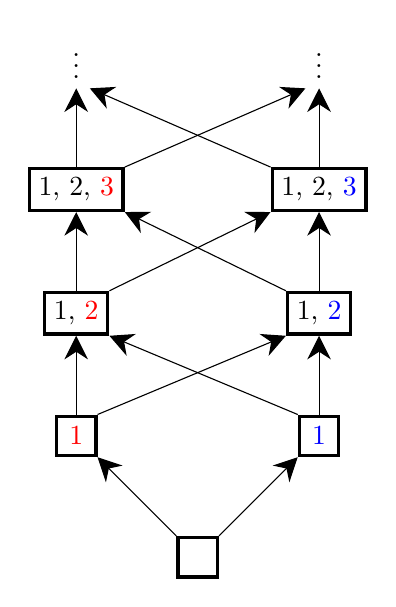
\begin{tikzpicture}[squarednode/.style={rectangle, draw, very thick, minimum size=5mm}]
			\node[squarednode]      (0)   [] {$ $};
			\node[squarednode]      (1r)   [above right=of 0] {{\color{blue}$1$}};
			\node[squarednode]      (1l)   [above left=of 0] {{\color{red}$1$}};
			\node[squarednode]      (2r)   [above=of 1r] {{1, \color{blue}$2$}};
			\node[squarednode]      (2l)   [above=of 1l] {{1, \color{red}$2$}};
			\node[squarednode]      (3r)   [above=of 2r] {{1, 2, \color{blue}$3$}};
			\node[squarednode]      (3l)   [above=of 2l] {{1, 2, \color{red}$3$}};
			\node      (4r)   [above=of 3r] {{$\vdots$}};
			\node      (4l)   [above=of 3l] {{$\vdots$}};
			\draw[-{Stealth[length=3mm, width=3mm]}, color=black] (0.north east) -- (1r.south west);
			\draw[-{Stealth[length=3mm, width=3mm]}, color=black] (0.north west) -- (1l.south east);
			\draw[-{Stealth[length=3mm, width=3mm]}, color=black] (1r.north) -- (2r.south);
			\draw[-{Stealth[length=3mm, width=3mm]}, color=black] (1l.north) -- (2l.south);
			\draw[-{Stealth[length=3mm, width=3mm]}, color=black] (1l.north east) -- (2r.south west);
			\draw[-{Stealth[length=3mm, width=3mm]}, color=black] (1r.north west) -- (2l.south east);
			\draw[-{Stealth[length=3mm, width=3mm]}, color=black] (2r.north) -- (3r.south);
			\draw[-{Stealth[length=3mm, width=3mm]}, color=black] (2l.north) -- (3l.south);
			\draw[-{Stealth[length=3mm, width=3mm]}, color=black] (2l.north east) -- (3r.south west);
			\draw[-{Stealth[length=3mm, width=3mm]}, color=black] (2r.north west) -- (3l.south east);
			\draw[-{Stealth[length=3mm, width=3mm]}, color=black] (3r.north) -- (4r.south);
			\draw[-{Stealth[length=3mm, width=3mm]}, color=black] (3l.north) -- (4l.south);
			\draw[-{Stealth[length=3mm, width=3mm]}, color=black] (3l.north east) -- (4r.south west);
			\draw[-{Stealth[length=3mm, width=3mm]}, color=black] (3r.north west) -- (4l.south east);
		\end{tikzpicture}
	\end{center}
	\caption{Counter-model to $\varphi$.}
	\label{fig1}
\end{wrapfigure}
\begin{example}
	Consider $\varphi = \neg(\neg \forall xA(x)\vee\neg \forall xB(x))$. There is a counter-model as shown in Figure~\ref{fig1},
	where we indicate at each world the elements that exist at it. For black numbers $n$, both $A(n)$ and $B(n)$ hold at that world, for red ones only $A(n)$, for blue ones only $B(n)$. The arrows indicate the order. $\neg\forall xA(x)$ is not fulfilled at worlds in the left column and $\neg\forall xB(x)$ is not fulfilled at worlds in the right column. In particular applying $f_{\neg \forall xA(x)}$ we must always reach the right column and applying $f_{\neg \forall xB(x)}$ we must always reach the left column. Therefore applying $f_{\neg \forall xA(x)}\circ f_{\neg \forall xB(x)}$ we cannot remain stationary.
\end{example}

Let us add that Lemma~\ref{thm:fo-countermodel-reduction} still equips us with additional information that could be used to guide proof search: We could add additional axioms that restrict the interpretation of functions. That is, we may assume that $f_\psi(w) = w$, if $\exists u(w = f_\psi(u))$ for all $\psi\in\mathcal F_\forall$ (i.e. that $f_\psi$ is idempotent), and $f_\psi(w) = w$, if $\exists u(w \geq f_\psi(u))$ for all $\psi\in\mathcal F_\to$ (which is even stronger than idempotence).
How adding such axioms impacts proof search will need to be evaluated in experiments.

\section{Conclusion}

We have presented embeddings of intuitionistic into classical logic for the propositional and the predicate case.
The transformation saw an exponential blow-up parameterized by $|\mathcal F_\to|$ in the propositional case and a complexity increase reflected by an arity-increase of one for all relations and the introduction of new function symbols in the predicate case.
A key motivation for our work is the potential of leveraging classical provers for showing intuitionistic validity.
%The practical feasibility of our translation is yet to be tested.
%In particular in the first-order case it is difficult to estimate how the increased complexity of the output formula impacts proof search.
Initial tests show promise but we plan on conducting a more thorough evaluation using state-of-the art automated theorem provers, in particular the Vampire theorem prover~\cite{kovacs2013first}.
A key factor yet to be determined is how large the parameters $|\mathcal F_\to|$ in the propositional case and $|\mathcal F|$ in the predicate case are in practice.

The above mentioned complexity considerations are direct consequences of our straightforward constructions.
We plan to establish better bounds in future work by utilizing structural properties of the input formula, in particular by constructing smaller counter-examples $\mathcal M_T$ in case certain atoms are independent from each other.
On the theoretical side, we also hope to give a new translation from QBF to IPC that improves our understanding of the relationship between intuitionistic propositional logic and the polynomial hierarchy.

Finally, we plan to complement the counter-model translation presented in this paper by a proof translation.
We will target the particular calculi used by state-of-the-art provers, e.g. superposition in the case of Vampire. Ultimately we hope that this will also open a new path for program extraction via the Curry--Howard Correspondence.

\bibliographystyle{splncs04}
\bibliography{bibliography}

\appendix

\section{Omitted content}

\begin{lemma}\label{ap1}
Let $\chi$ be a formula and let $\{z_1\dots z_n\} = Z$ contain all free variables in $\chi$, then for every structure $\mathcal M = (M, I)$ there exists $\mathcal M_\chi = (M, I_\chi$) such that $p^{I_{\chi}} = p^I$ for all function and relation symbols $p$ occurring in $\chi$ and for all variable assignments $v$ we have
	\begin{itemize}
		\item if $M, v \models\chi$ then $\mathcal M_\chi, v\models\chi^S_T$.
		\item if $\mathcal M, v\not\models\chi$ then $\mathcal M_\chi, v\not\models\chi^H_T$.
	\end{itemize}
\end{lemma}

\begin{proof}
	We proceed by simultaneous induction on the formula height.
	
	For atomic $\chi$ the claims are clear.
	
	Otherwise there are $3$ cases:
	
	1. $\chi = \varphi\circ\psi$ for $\circ\in\{\wedge,\vee,\to\}$. By induction hypothesis there exist $\mathcal M_{\varphi, v} = (M, I_{\varphi, v})$ and $\mathcal M_{\psi, v} = (M, I_{\psi, v})$ for $\varphi,\psi$ as stated in the lemma.
Then we can define $I_{\chi, v}$ as follows:
	
	For every symbol $p$ that occurs in $\varphi^S_Z$ or $\varphi^H_Z$ but not $\psi^S_Z, \psi^H_Z$, we set $p^{I_{\chi, v}} = p^{I_{\varphi, v}}$. For every symbol $p$ that occurs in $\psi^S_Z$ or $\psi^H_Z$ but not $\varphi^S_Z, \varphi^H_Z$, we set $p^{I_{\chi, v}} = p^{I_{\psi, v}}$. Otherwise $p$ already occurs in $\varphi$ so have $p^{I_{\chi, v}} = p^I$.
	
	Let $\circ=\ \to$. Suppose $\mathcal M, v\models\chi$. Then $\mathcal M, v\not\models\varphi$ or $\mathcal M\models\psi$ and therefore $\mathcal M_\chi\not\models\varphi^S_Z$ or $\mathcal M_\chi\models\psi^H_Z$, i.e. $\mathcal M_\chi\models\chi^S_Z$. On the other hand suppose $\mathcal M, v\not\models\chi$. Then $\mathcal M, v\models\varphi$ and $\mathcal M, v\not\models\psi$ and therefore $\mathcal M_\chi, v\models \varphi^S_Z$ and $\mathcal M_\chi, v\not\models\psi^S_Z$, i.e. $\mathcal M_\chi\not\models\chi^H_Z$. Analogous arguments work for $\circ\in\{\wedge, \vee\}$.
	
	2. $\chi = \forall x\varphi$. Choose $s^{I_\chi}:M^n\to M$ such that $s^{I_\chi}(x_1,\dots, x_n) = m$ if there exists $m\in M$ such that $\mathcal M, v[x_1/z_1\dots x_n/z_n, m/a]\not\models\varphi[a/x]$ for all $v$ and arbitrary otherwise. Since $Z$ contains all free variables occurring in $\chi$ this is a well-defined function.
	
By induction hypothesis there exists a structure $\mathcal M_{\varphi[a/x]}$ as is the Lemma. Let $p^{I_\chi} = p^{I_{\varphi[a/x]}}$ for all symbols occurring in $\chi$ and $$p^{I_\chi}(x_1\dots x_{i-1}, x_{i+1}\dots x_m) = p^{I_{\varphi[a/x]}}(x_1\dots x_{i-1}, s^{I_\chi}(x_1\dots x_n), x_{i+1}\dots x_m)$$ for all symbols $p$ occurring in $\varphi[a/x]^S_{Z\cup a}$ or $\varphi[a/x]^H_{Z\cup a}$ but not in $\chi$ where $x_i$ is the argument corresponding to the free variable $a$.
	
Suppose $\mathcal M, v\models\chi$. Then, for all $m\in M$ we have that $\mathcal M, v[m/a]\models\varphi[a/x]$ and therefore $\mathcal M_{\chi}, v[m/a]\models\varphi[a/x]^S_{Z\cup\{a\}}$ and thus $\mathcal M_{\chi}, v\models \forall x\varphi([a/x]^S_{Z\cup\{a\}}[x/a])$, i.e. $\mathcal M_\chi,v\models \chi^S_Z$. On the other hand suppose $\mathcal M, v\not\models\chi$. Then there exists $m\in M$ such that $\mathcal M, v[m/a]\not\models\varphi[a/x]$ and therefore $\mathcal M_\chi, v[m/a]\not\models\varphi[a/x]^H_{Z\cup\{a\}}$ and so by definition $\mathcal M_\chi, v\not\models\varphi[s(z_1,\dots z_n)/x]^H_Z$, i.e. $\mathcal M_\chi, v\not\models(\forall x\varphi)^H_Z$.
	
	3. $\chi = \exists x\varphi$. The argument runs dually to 2. Choose $s^{I_\chi}:M^n\to M$ such that $s^{I_\chi}(x_1,\dots, x_n) = m$ if there exists $m\in M$ such that for all $v$ we have $\mathcal M, v[x_1/z_1\dots x_n/z_n, m/a]\models\varphi[a/x]$ and arbitrary otherwise. Since $Z$ contains all free variables occurring in $\chi$ this is a well-defined function.
	
	By induction hypothesis there exists a structure $\mathcal M_{\varphi[a/x]}$ as is the Lemma. Let $p^{I_\chi} = p^{I_{\varphi[a/x]}}$ for all symbols occurring in $\chi$ and $$p^{I_\chi}(x_1\dots x_{i-1}, x_{i+1}\dots x_m) = p^{I_{\varphi[a/x]}}(x_1\dots x_{i-1}, s^{I_\chi}(x_1\dots x_n), x_{i+1}\dots x_m)$$ for all symbols $p$ occurring in $\varphi[a/x]^S_{Z\cup a}$ or $\varphi[a/x]^H_{Z\cup a}$ but not in $\chi$ where $x_i$ is the argument corresponding to the free variable $a$.
	
	Then as in 2 from $\mathcal M, v\models \chi$ follows $\mathcal M_\chi,v\models\chi^S_Z$ and from $\mathcal M, v\not\models \chi$ follows $\mathcal M_\chi,v\not\models\chi^H_Z$.
\end{proof}

\begin{lemma}\label{ap2}
	For every structure $\mathcal M$ and $\{z_1\dots z_n\} = Z$ that contains all free variables in $\chi$ and variable assignment $v$
	\begin{itemize}
		\item if $\mathcal M, v\models\varphi^S_Z$ then $\mathcal M, v\models \varphi$
		\item if $\mathcal M, v\not\models\varphi^H_Z$ then $\mathcal M, v\not\models\varphi$.
	\end{itemize}
\end{lemma}

\begin{proof}
	Again we proceed by simultaneous induction on the formula height.
	
	For atoms the claims are clear. We distinguish 5 cases.
	
	1. $\chi = \varphi\to\psi$. Suppose $\mathcal M, v\models\chi^S_Z$, i.e. $\mathcal M, v\not\models\varphi^H_Z$ or $\mathcal M, v\models\psi^S_Z$. By induction hypothesis $\mathcal M, v\not\models \varphi$ or $\mathcal M, v\models\psi$, i.e. $\mathcal M, v\models \chi$. On the other hand suppose $\mathcal M, v\not\models\chi^H_Z$, i.e. $\mathcal M, v\models\varphi^S_T$ and $\mathcal M, v\not\models\varphi^H_Z$. Again by induction hypothesis $\mathcal M,v\models\varphi$ and $\mathcal M, v\not\models \varphi$, so $\mathcal M, v\not\models\chi$.
	
	2. + 3. Conjunctions and Disjunctions are dealt with analogously.
	
	4. $\chi = \forall x\varphi$.  Suppose $\mathcal M, v\models\chi^S_Z$, i.e. for all $m\in M$ we have $\mathcal M, v[m/a]\models \chi[a/x]^S_{Z\cup\{a\}}$ and by induction hypothesis $\mathcal M, v[m/a]\models \chi[a/x]$. Then it follows that $\mathcal M, v\models\varphi$. On the other hand suppose $\mathcal M, v\not\models\chi^H_Z$, i.e. there exists $m\in M$ such that $\mathcal M, v[m/a]\not\models\chi[a/x]^H_{Z\cup \{a\}}$, then by induction hypothesis $\mathcal M, v[m/a]\not\models \chi[a/x]$, i.e. $\mathcal M, v\not\models\forall x\chi$.
	
	5. $\chi = \exists x\varphi$.  The argument runs dually to 4.
\end{proof}

\begin{definition}\label{def:transf-structure}
	For every classical and intuitionistic structure $\mathcal M$ define a structure $\mathcal S(\mathcal M,\varphi)$ that agrees with $\mathcal M$ on everything except the interpretation(s) of atoms of the form $P_\psi$. By slight abuse of notation we denote with $\vec z_\psi$ elements of the domain instead of variables. In the classical case, we set
	$$\begin{matrix}
		P_A^I(\vec z_A):\Leftrightarrow A^I(\vec z_A)\\
		P_{\varphi\wedge\psi}^I(\vec z_{\varphi\wedge\psi}) :\Leftrightarrow P_{\varphi}^I(\vec z_\varphi)\wedge P_{\psi}^I(\vec z_\psi)\indent P_{\varphi\vee\psi}^I(\vec z_{\varphi\vee\psi}) :\Leftrightarrow P_{\varphi}^I(\vec z_\varphi)\vee P_{\psi}^I((\vec z_\psi))\\P_{\varphi\to\psi}^I(\vec z_{\varphi\to\psi}) :\Leftrightarrow (\neg P_{\varphi}^I(\vec z_{\varphi}))\vee P_{\psi}^I(\vec z_{\psi})\\P_{\forall x\varphi}^I(\vec z_{\forall x\varphi}) :\Leftrightarrow \{\vec z\:|\:\:P_{\varphi}^I(\vec z_\varphi) \text{ for all $x\in M$}\}\indent P_{\exists x\varphi}^I(\vec z_{\exists x\varphi}) :\Leftrightarrow \{\vec z\:|\:\:P_{\varphi}^I(\vec z_\varphi) \text{ for some $x\in M$}\},
	\end{matrix}$$
	and for intuitionistic logic and each world $u$, we set
	$$\begin{matrix}
		P_A^{I_u}(\vec z_A):\Leftrightarrow A^{I_u}(\vec z_A)\\
		P_{\varphi\wedge\psi}^{I_u}(\vec z_{\varphi\wedge\psi}) :\Leftrightarrow P_{\varphi}^{I_u}(\vec z_\varphi)\wedge P_{\psi}^{I_u}(\vec z_\psi)\indent P_{\varphi\vee\psi}^{I_u}(\vec z_{\varphi\vee\psi}) :\Leftrightarrow P_{\varphi}^{I_u}(\vec z_\varphi)\vee P_{\psi}^{I_u}((\vec z_\psi))\\
		P_{\varphi\to\psi}^{I_u}(\vec z_{\varphi\to\psi}) :\Leftrightarrow(\neg P_{\varphi}^{I_w}(\vec z_{\varphi}))\vee P_{\psi}^{I_w}(\vec z_{\psi})\text{ for all $w\geq u$}\\
		P_{\forall x\varphi}^{I_u}(\vec z_{\forall x\varphi}) :\Leftrightarrow P_{\varphi}^{I_w}(\vec z_\varphi) \text{ for all $w\geq u$, $x\in M_w$}\indent P_{\exists x\varphi}^{I_u}(\vec z_{\exists x\varphi}) :\Leftrightarrow P_{\varphi}^{I_u}(\vec z_\varphi) \text{ for some $x\in M_u$}.
	\end{matrix}$$
\end{definition}

Lemmas~\ref{thm:struct1} and~\ref{thm:struct2} then follow directly by induction on the height of $\varphi$.

\begin{lemma}\label{proof:first-order-normal-form}
	For every predicate formula $\varphi$ there exists a nullary relation symol $P$ as well as sets of clauses $\mathcal R$ of the form
	$$\forall \vec x\left(\bigwedge_i A_i\to \bigvee_j B_j\right)$$
	called \emph{flat} clauses and $\mathcal X$ of the form
	$$\forall \vec x\left((A\to B)\to C\right)$$
	called \emph{implication} clauses as well as $\mathcal Q$ of the form
	$$\forall\vec x\left((\forall y A)\to B\right)$$
	called \emph{quantification} clauses such that $\varphi$ is intuitionistically equivalid to
	$$\left(\bigwedge\mathcal R\wedge\bigwedge \mathcal X\wedge\bigwedge\mathcal Q\right)\to P$$where $A_i, B_i, A, B, C$ are atomic. This size of $\mathcal R, \mathcal X, \mathcal Q$ is linear in the size of $\varphi$. In general this formula will contain new function symbols and relational symbols.
\end{lemma}

\begin{proof}
	As in~\cite{otten2005clausal} we may assume that $\varphi$ is of the form $\psi\to P$. Recall that the transformation works by transforming $\psi$ into a set of equivalent assumptions $\left\lbrack \psi\right\rbrack$ of the desired form. We extend the given procedure with rules for quantifiers as follows:
	\begin{align*}
		\left\lbrack(\forall x \psi)\to A\right\rbrack&:= \left\lbrack\psi[s(\vec z)/x]\to A\right\rbrack\\
		\left\lbrack A\to (\forall x\psi)\right\rbrack&:= \{\forall x\chi[x/a]\:|\:\chi\in\left\lbrack A\to\psi[a/x]\right\rbrack\}\\
		\left\lbrack(\exists x\psi)\to A\right\rbrack&:= \{\forall x\chi[x/a]\:|\:\chi\in\left\lbrack A\to\psi[a/x]\right\rbrack\}\\
		A\to (\exists x\psi)&:= \left\lbrack A\to\psi[s(\vec z)/x]\right\rbrack
	\end{align*}
	where $s$ is a new function symbol, $a$ is a new free variable and $\vec z$ ranges over the free variables in $\psi$.
	While the generated set of clauses is in general not equivalent to $\psi$, section~\ref{section:herbrandiaztion} guarantees that it is at least equivalid.
\end{proof}

\begin{lemma}~\label{proof:prop-countermodel-reduction}
	Let $\mathcal M = (M, I)$ be a counter-model to $\mathcal \varphi^{CH}$.
	\begin{enumerate}
		\item $\psi$ is fulfilled at $f_{[\psi]}^I(m)$ for all $m\in M, \psi\in\mathcal X$.
		\item If $\psi$ is fulfilled at some $m\in M$ then $\psi$ is fulfilled at all $n\geq m$.
	\end{enumerate}
\end{lemma}

\begin{proof}
	1. If $C^I(m)$ is true then we are done due to persistency. Otherwise $C^I(m)$ is false.
	Because $(A^I(f_{[\psi]}^I(m))\to B^I(f_{[\psi]}^I(m)))\to C^I(u)$ holds, then $A^I(f_{[\psi]}^I(u))\to B^I(f_{[\psi]}^I(u))$ must be false.
	
	
	2. Let $n$ be some element with $n\geq m$.
	If $C^I(n)$ is true, we are done.
	Otherwise $C^I(n)$ is false.
	Due to persistency $C^I(m)$ is also false.
	Because $\psi$ is fulfilled at $m$, $A^I(m)\to B^I(m)$ must be false, i.e. $A^I(m)$ is true and $B^I(m)$ is false. Then $A^I(n)$ and $A^I(f^I_{[\psi]}(n))$ are also true due to persistency.
	Because $(A^I(f^I_{[\psi]}(n))\to B^I(f^I_{[\psi]}(n)))\to C^I(n)$ holds, we now get that  $B^I(f^I_{[\psi]}(n))$ must be false.
	But then due to persistency so is $B^I(n)$ and we have that $\psi$ is fulfilled at $n$.
\end{proof}

\begin{example}\label{ex:prop-tree-model}
	This is an example for the model translation from Corollary~\ref{cor:prop-tree-model}. Consider
	$$\mathcal S = \{(A\to B)\to C, (B\to A)\to D, (A\wedge B)\to \bot, (C\vee D)\to E\}$$and $\varphi = \bigwedge S\to E$ which has the Kripke counter-model, depicted below,
	\begin{center}
		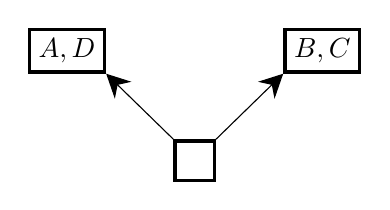
\begin{tikzpicture}[squarednode/.style={rectangle, draw, very thick, minimum size=5mm}]
			\node (center) {};
			\node[squarednode]      (right)   [right=of center] {$B, C$};
			\node[squarednode]      (left)    [left=of center] {$A, D$};
			\node[squarednode]      (lower)       	[below=of center] {};
			\draw[-{Stealth[length=3mm, width=3mm]}] (lower.north west) -- (left.south east);
			\draw[-{Stealth[length=3mm, width=3mm]}] (lower.north east) -- (right.south west);			
		\end{tikzpicture}
	\end{center}
	\vspace*{-.3cm}where at each node the true propositions are indicated.
	%	
	There is a corresponding classical counter-model $\mathcal M = (M, I)$ to $\varphi^\circ$ with $M = \{u, u_l, u_r\}$, $A^{I}(l) = D^I(l) = B^I(r) = C^I(r) = 1$ and $0$ else.
	%
	Denoting $\psi_1 := (A\to B)\to C$ and $\psi_2 := (B\to A)\to D$, this corresponds to a transformed counter-model $\mathcal M_T = (M_T, I_T)$ of $\varphi^\circ$ with $M_T = \{\epsilon, \psi_1, \psi_2, \psi_1\psi_2, \psi_2\psi_1\}$ and interpretation as presented below:
	\begin{center}
		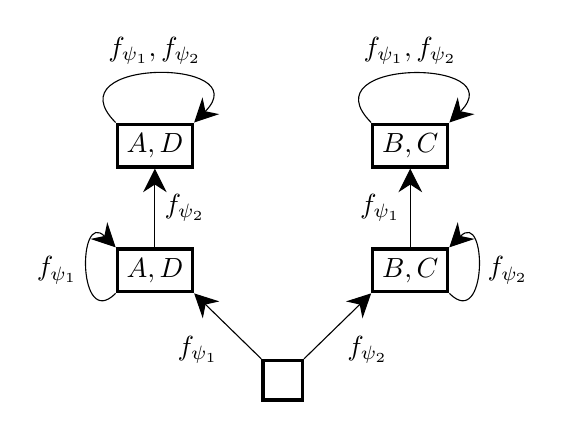
\begin{tikzpicture}[squarednode/.style={rectangle, draw, very thick, minimum size=5mm}]
			\node (center) {};
			\node[squarednode]      (right1)   [right=of center] {$B, C$};
			\node[squarednode]      (right2)   [above=of right1] {$B, C$};
			\node[squarednode]      (left1)    [left=of center] {$A, D$};
			\node[squarednode]      (left2)    [above=of left1] {$A, D$};
			\node[squarednode]      (lower)       	[below=of center] {};
			\draw[-{Stealth[length=3mm, width=3mm]}] (lower.north west) -- (left1.south east) node [midway, below left] {$f_{\psi_1}$};
			\draw[-{Stealth[length=3mm, width=3mm]}] (lower.north east) -- (right1.south west) node [midway, below right] {$f_{\psi_2}$};
			\draw[-{Stealth[length=3mm, width=3mm]}] (left1.north) -- (left2.south) node [midway, right] {$f_{\psi_2}$};
			\draw[-{Stealth[length=3mm, width=3mm]}] (right1.north) -- (right2.south) node [midway, left] {$f_{\psi_1}$};
			\draw[-{Stealth[length=3mm, width=3mm]}] (left1.south west) to [out=225, in=135, loop, looseness=3] node [left] {$f_{\psi_1}$} (left1.north west);		
			\draw[-{Stealth[length=3mm, width=3mm]}] (right1.south east) to [out=315, in=45, loop, looseness=3] node [right] {$f_{\psi_2}$} (right1.north east);
			\draw[-{Stealth[length=3mm, width=3mm]}] (left2.north west) to [out=135, in=45, loop, looseness=3] node [midway, above] {$f_{\psi_1}, f_{\psi_2}$} (left2.north east);
			\draw[-{Stealth[length=3mm, width=3mm]}] (right2.north west) to [out=135, in=45, loop, looseness=3] node [midway, above] {$f_{\psi_1}, f_{\psi_2}$} (right2.north east);		
		\end{tikzpicture}
	\end{center}
\end{example}


\begin{lemma}\label{lemma:QBF}
	$\varphi$ is not intuitionistically valid iff $\varphi^Q$ is a satisfiable QBF.
\end{lemma}
\begin{proof}
Suppose $\varphi$ is not intuitionistically valid.
Then, $(\bigwedge R\wedge\bigwedge X)\to P$ has an intuitionistic counter-model. By the previous section there exists a classical counter-model $\mathcal M$ for $\bigwedge\mathcal S^\#\to P^\epsilon$.
We now define a QBF model iteratively.
For each atom $A$ interpret $A^0$ such as $\mathcal M$ interprets $A^\epsilon$. Suppose we are given interpretations of all atoms $A^i$ for $i < n$ and a sequence with no repetitions $\psi_1\dots\psi_{n-1}$ over $\mathcal F_\to$ such that $\psi_i$ is exactly the $\psi\in\mathcal F_\to$ for which $F_{\psi}^i$ is true and $A^i$ is interpreted as $A^{\psi_1\dots\psi_i}$  in $\mathcal M$.
Let the $X^{n}_\psi$ be arbitrarily interpreted (since they are $\forall$-quantified). If not exactly one of the $X^{n}_\psi$ is interpreted as true, then valid$(n)$ fails and the remaining propositions can be chosen arbitrarily. If $X^i_{\psi_n} = 1$ for some $i < n$, then valid$(n)$ also fails and the remaining propositions can be chosen arbitrarily.
So we may assume that $\psi_1\dots\psi_n$ is a sequence with no repetitions.
Interpret the atoms $A^n$ as $\mathcal M$ interprets $A^{\psi_1\dots\psi_n}$.
Continue this construction until $n  = |\mathcal X|$. Then from $\mathcal M$ being a counter-example to $\bigwedge\mathcal S^\#\to P^\epsilon$ it directly follows that this interpretation satisfies $\varphi^Q$.
	
	On the other hand suppose $\varphi^Q$ is satisfiable. We construct a counter-example to $\varphi^\#$.
	Again we proceed iteratively. Interpret $A^\epsilon$ such as $A^0$ is interpreted in some satisfying interpretation of $\varphi^Q$. Suppose we are given a sequence $\psi_1\dots \psi_{n-1}$ such that for $i<n$ having $A^i = A^{\psi_0\dots\psi_{n-1}}$ is part of a satisfying interpretation of $\varphi^Q$, in which $X^i_\psi$ is chosen true iff $\psi = \psi_i$. Let $\psi_n\in\mathcal X$. Consider some interpretation of the $A^n$ that are part of a satisfying assignment where $X^n_\psi$ is true iff $\psi = \psi_n$ and all variables quantified above are chosen as before. Have $A^{\psi_0\dots\psi_n} = A^n$ for each propositional variable $A$. From the definitions it directly follows that construction yields a counter-model for $\varphi^\#$.
\end{proof}

\begin{lemma}\label{proof:fo-simplification}
	$\varphi$ is intuitionistically valid if and only of $\varphi'$ is classically valid.
\end{lemma}

\begin{proof}
	We proceed by translation of counter-examples. Suppose first we have a counter-example $\mathcal M = (M, I)$ to $\varphi'$. As a Kripke frame $(W, \leq)$ take all $ W = \{m\in M\:|\:\text{ World}^I(m)\}$ let $\leq$ be $\preceq^I$ restricted to $W$. Then let $M_u = \{m\in M\:|\: E(m, u)\}$ and let $f^{I_u}$ be $f^I$ restricted to $M_u$ and $A^{I_u}(\vec x): \Leftrightarrow A^\#(\vec x, u)$. It is then a straightforward check of definitions that this defines a Kripke counter-model to $\varphi$.
	
	The other direction is a bit more involved. Suppose we have a Kripke counter-model to $\varphi$ with frame $(W, \preceq)$ and family of $\Sigma$-structures $(M_w, I_w)_{w\in W}$. In particular since it is a counter-model there exists $w_0\in W$ with $w_0\not\models\varphi$. Let $W_0 = \{w\in W\:|\: w\geq w_0\}$ and define an equivalence relation $\sim$ on $\{(x, u)\:|\:u\in W_0, x\in M_u\}$ via $(x, u)\sim (y, w)$ iff $x = y$ and there exists $v\in W_0$ comparable with both $u, w$ such that $x\in v$ and denote the equivalence class of $(x, u)$ with $[x, u]$. Let $M = W_0\cup \{[x, u]\:|\:u\in W_0, x\in M_u\}$.
	Now have
	\begin{itemize}
		\item $s^I = w_0$.
		\item $E^I(m, w)$ iff $w\in W_0$ and $m \sim [x, w]$ for some $x\in M_w$.
		\item $f^I(m_1\dots m_n) =\begin{cases}
			f^{I_u}(x_1\dots x_n), &\text{if there are $ u\in W_0, x_i\in M_u$ with $m_i\sim [x_i, u]$ for all $i$,}\\
			w_0, & \text{otherwise.}
		\end{cases}$
		\item ${A^\#}^I(m_1\dots m_n, u) \Leftrightarrow\begin{cases}
			A^{I_u}(x_1\dots x_n), &\text{if $u\in W_0$ and $\exists x_i\in M_u$ w. $m_i\sim [x_i, u]$ for all $i$,}\\
			\top, & \text{otherwise.}
		\end{cases}$
	\end{itemize}
	One easily verifies that these are well-defined. Let us now briefly check that this indeed defines a counter-model. First of all ${P^\#}^I(s^I)$ is false since $P^{I_{w_0}}$ is. Clearly World$(w_0)$ holds and $K(\varphi)$ is also easily verified. All that remains to show is $M, I\models\bigwedge\mathcal S'$. Consider e.g. the case where $\psi\in\mathcal S$ is of the form
	$$ \forall \vec z((A(\vec a)\to B(\vec b))\to C(\vec c))$$
	We have to show that
	$$M, I\models \forall \vec z\forall u(\vec E(t, u)\to \forall w(u\preceq w\to A^\#(\vec a, w)\to B^\#(\vec b, w))\to C^\#(\vec c, u))$$
	holds. Suppose towards contradiction that it does not, i.e. there are $u, \vec z\in M$ such that for all $w\in M$
	$$\vec E^I(\vec z, u)\to (u\preceq w\to {A^\#}^I(\vec a, w)\to {B^\#}^I(\vec b, w))\to {C^\#}^I(\vec c, u)$$ is false. For that ${C^\#}^I(\vec c, u)$ must be false and in particular $u\in W_0$. Futhermore $\vec E^I(\vec z, u)$ must be true and we can write $\vec z = [z_1, u]\dots[z_n, u]$ for some $z_i\in W_u$. Note that the above is false in particular for $w\in M_0$ with $u\preceq w$. But this would imply
	$$((A^{I_u}(\vec a)\to B^{I_u}(\vec b))\to C^{I_u}(\vec c))[\vec z/z_1\dots z_n]$$in our original Kripke counter-model. The other cases are analogous.
\end{proof}

\end{document}
